%!TEX root = thesis.tex

\chapter{Data Visualization}
\label{chapter:dataviz}

\section{Definition}

According to \citet[chap.~3]{kosara_visualization_2007}, there is no universally accepted definition of visualization. He proposes the following for a ``minimal set of requirements for any visualization'':

\begin{itemize}
	\item It is based on (non-visual) data
	\item It produces an image
	\item The results are readable and recognizable
\end{itemize}

According to him, while visualizations can also have other properties or qualities, such as interaction or visual efficiency, the requirements above are the ones needed for technical definition of the term. Moreover, it should be emphasized that according to this definition, visualization is the \emph{process} itself, not the result of it.

\citet[chap.~4]{kosara_visualization_2007} argues that visualization is separated into two types, \emph{pragmatic} and \emph{artistic} visualization. \fixme{This is related to Hassenzahl's UX definition. May be nice to refer to that as well somewhere.} Pragmatic visualization focuses on the analysis of the data in order to show its relevant characteristics as efficiently as possible. Artistic visualization on the other hand concentrates on the communication of a concern, not the display of the actual data. Therefore, artistic visualizations may emphasize or even exaggerate some of the features of the data. \citeauthor{kosara_visualization_2007} states that while these types focus on the opposite sides of the visualization spectrum, it may be possible to close the gap using, e.g., interaction.

The first requirement for visualizations by \citet{kosara_visualization_2007} dictates that the visualization is based on data. This is in alignment with the principle of \citet{tufte_visual_1986} which states that visualizations should, above all else, show the data. This is an essential characteristic of \emph{data} visualizations: the visualization is a function which takes data as an input and produces a visual object as an output. In less technical terms, this means that the visualization turns data into visual, effortlessly and efficiently digestible format. \fixme{Comment by Sami: T�� on hyv� peruspointti, eli miksi visualisaatiota ylip��t��n tehd��n. Voisi ehk� laajentaa/tuoda enemm�n esiin.}

This leads to the fact that the data and visualization are not inherently tied to each other; the visualization ``function'' can be independent of the data and thus it may be possible to create a visualization framework or platform which is able to function on a potentially wide range of data.

\fixme{The goal of visualization is (usually) better understanding of the data.}

% This may need to moved to Thematic Map Visualization part:
% ``As this thesis concentrates on the display of data, the analysis of data is considered mainly outside the scope.''

\section{Principles for Successful Data Visualization}
\label{section:visualizationprinciples}

The requirements presented in the previous section are sufficient for the definition of data visualization. However, they do not convey any information about visualization quality. In order to discover the characteristics for successful data visualization, additional principles are needed. \citet[p.~13]{tufte_visual_1986} states that excellent graphics (i.e., results of visualizations) consist of ``complex ideas communicated with clarity, precision and efficiency''. In practice, this means that the graphics should emphasize the actual data and its nuances above everything else, while serving a clear purpose.

In addition to graphics principles presented in the previous paragraph, \citet[p.~93]{tufte_visual_1986} presents the concept of \emph{data-ink}. Data-ink represents the ink used for displaying the data in a visualization. He argues that in an excellent visualization, most, if not all, ink used should contribute to display of the data. However, research by \citet{inbar_minimalism_2007} suggests that maximizing the share of data-ink may not be beneficial to the user experience of the visualization: while, e.g., axis lines in a chart are not data-ink according to the definition of \citeauthor{tufte_visual_1986}, they may be beneficial to the user experience of the chart by providing visual structure.

The principles presented above are essential, but too abstract in order to be used as a sole basis for defining a good visualization. However, when combined with \citeauthor{kosara_visualization_2007}'s data visualization definition stated above, the principles become considerably more useful and concrete. \citet{azzam_j-b_2013} propose an adapted version of the definition by \citet{kosara_visualization_2007}: ``Data visualization is a process that (a) is based on qualitative or quantitative data and (b) results in an image that is representative of raw data, which is (c) readable by viewers and supports exploration, examination and communication of the data''. The most significant differences are that the definition complements the second requirement of \citeauthor{kosara_visualization_2007} (``It produces an image'') by requiring the produced image to represent the data truthfully, and requires the visualization to be enlightening instead of just readable. This definition effectively combines the definition by \citet{kosara_visualization_2007} with the principle of showing data introduced by \citet{tufte_visual_1986}. The adapted definition facilitates the process of creating a successful data visualizations by offering a more concrete version of Tufte's principles. It gives the developer of the visualization slightly more concrete checklist for representing the data: make sure the representation does not (a) omit or (b) overrepresent any information, and (c) helps the viewer gain knowledge \citep{azzam_j-b_2013}.

For the most concrete principles, \citet{zuk_heuristics_2006} provide a list of heuristics for visualizations established in perceptual, cognitive and usability research. The list combines several heuristics from multiple heuristics sets by \citet{shneiderman_eyes_1996,zuk_theoretical_2006,amar_best_2004}. While the combination results in potentially conflicting or redundant heuristics, it nevertheless results in a concrete checklist for making successful visualizations. The heuristics are presented below.

\begin{enumerate} \itemsep1pt \parskip0pt \parsep0pt
	\item Ensure visual variable has sufficient length
	\item Don't expect a reading order from color
	\item Color perception varies with size of colored item
	\item Local contrast affects color
	\item Consider people with color blindness
	\item Preattentive benefits increase with field of view
	\item Quantitative assessment requires position or size variation
	\item Preserve data to graphic dimensionality
	\item Put the most data in the least space
	\item Remove the extraneous (ink)
	\item Consider Gestalt Laws
	\item Provide multiple levels of detail
	\item Integrate text wherever relevant
	\item {[}Provide{]} overview first
	\item Zoom and filter [out uninteresting data]
	\item {[}Provide{]} details on demand
	\item Relate (consider relationships among items)
	\item Extract (allow extraction of data and its subsets)
	\item {[}Keep{]} history [of actions]
	\item Expose uncertainty
	\item Concretize relationships
	\item Determination of Domain Parameters
	\item Multivariate Explanation
	\item Formulate cause \& effect
	\item Confirm Hypotheses
\end{enumerate}

\fixme{The list is ugly. Move to an appendix?}

\section{Visualizing Geographical Data}

As geographic data is associated with a specific location, the most natural way of visualizing it is by using a map \citep[chap.~1]{kraak_cartographic_1998,kraak_cartography_2011}. This technique is called \emph{thematic mapping} \citep[chap.~1]{slocum_thematic_2014}. Thematic mapping does not require any specific format of data, except for the geographical dimension \citep[chap.~1]{kraak_cartography_2011}. However, the nature of the data has a great effect on the method, or type, of thematic mapping.

\subsection{Methods for Thematic Mapping}
\label{subsection:mappingmethods}

As stated above, there are several types of geographical data, many of which are fundamentally different requiring different visualization methods. Therefore, several different thematic mapping methods have been developed. \citet[chap.~14-18]{slocum_thematic_2014} list some of the most typical ones:

\paragraph{Choropleth Map}

Choropleth maps are used primarily for visualizing data which coincides with predefined enumeration units. This method is most naturally used for situations when the enumeration units are directly linked to data results, such as votes in an election for each voting area. However, choropleth maps are also used to depict ``typical'' values for an area even when in reality, the area is heterogeneous in relation to the measured quality. Choropleth maps are commonly visualized grouping a specified area using a constant color or a common symbol. Figure \ref{fig:choropleth} depicts an example of a choropleth map. (Ibid.)

\begin{figure}[htbp]
  \begin{center}
    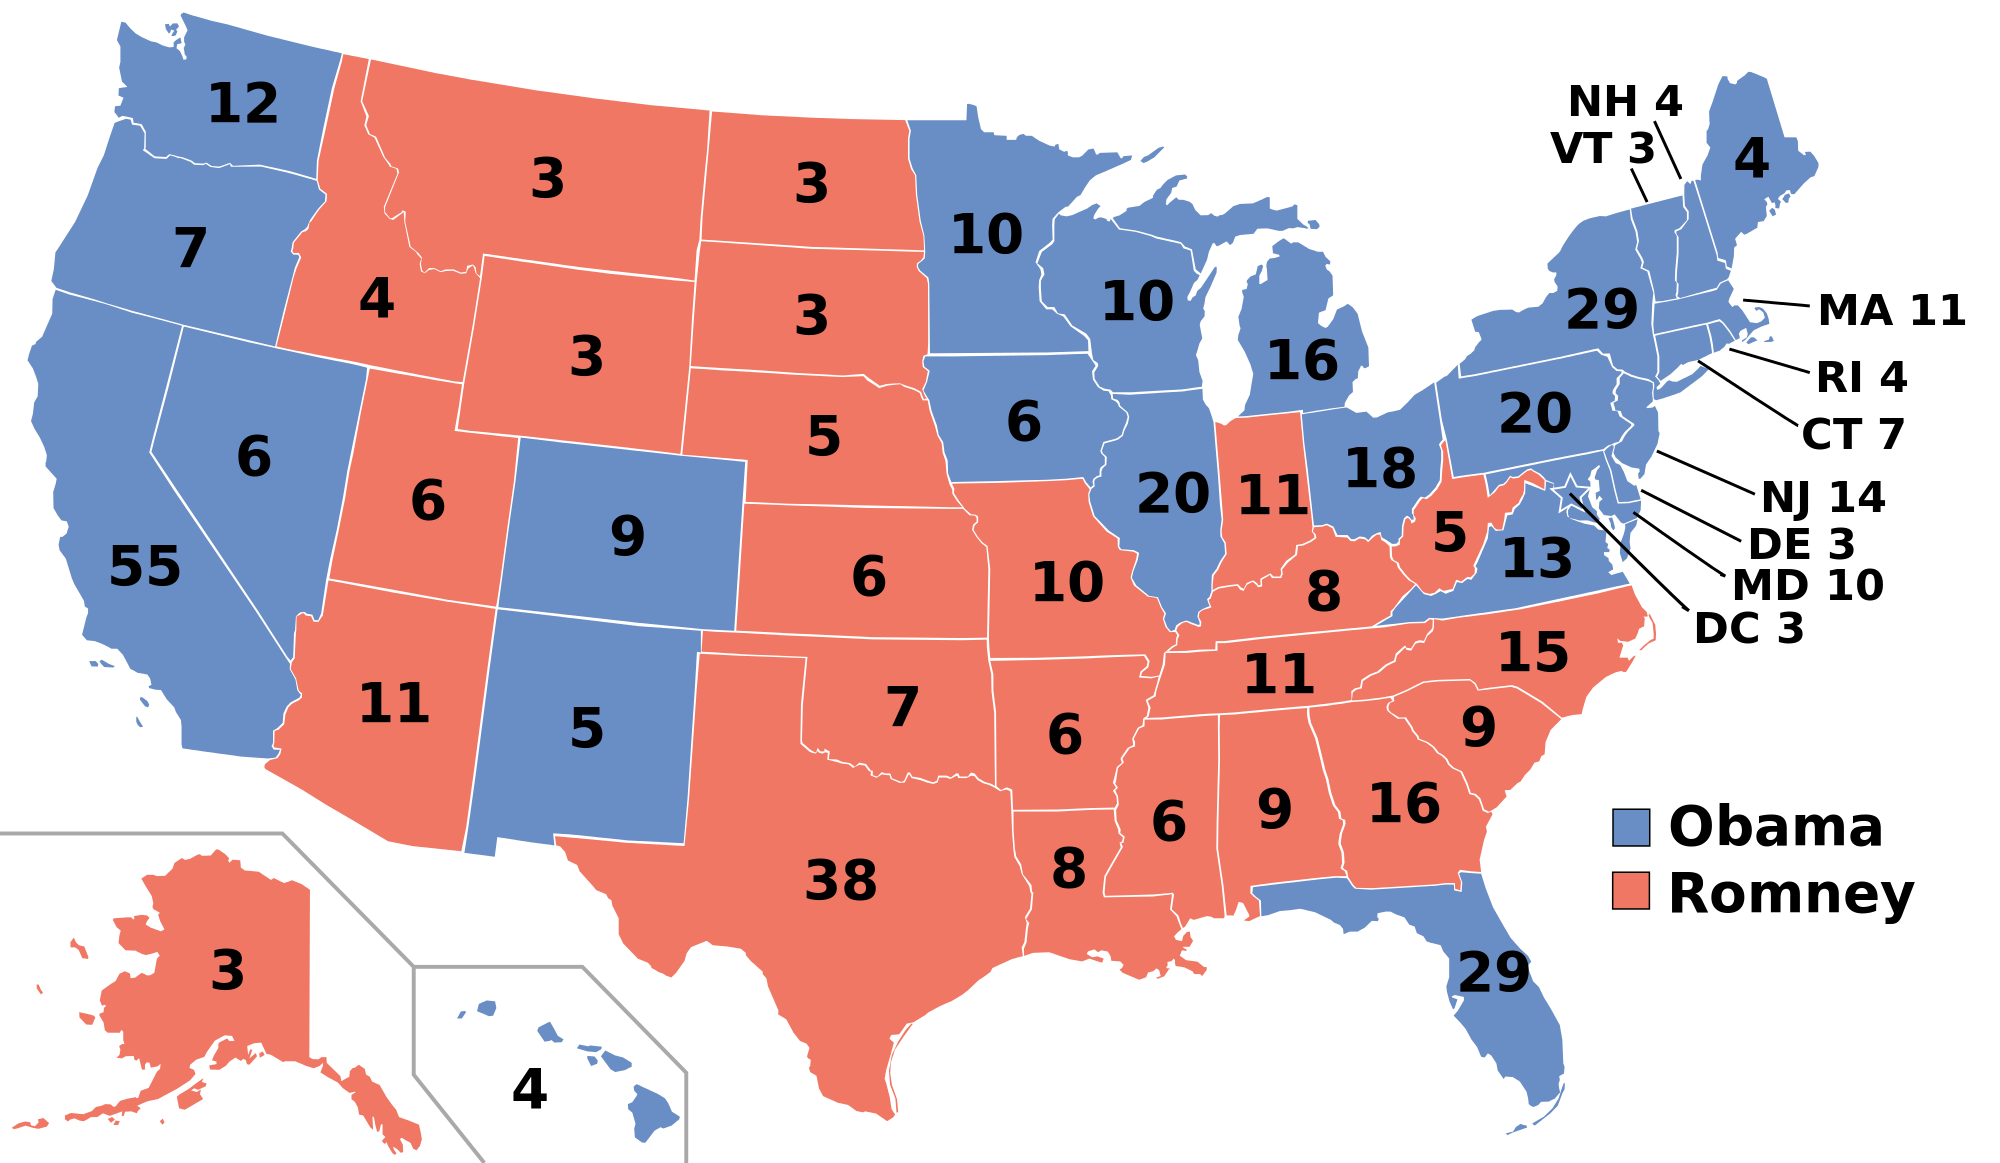
\includegraphics[width=8cm]{images/choropleth-example.png}
    \caption{A choropleth map depicting regional voter turnout in Finnish presidential elections of 2012}
    \label{fig:choropleth}
  \end{center}
\end{figure}

\paragraph{Isarithmic Map}

Isarithmic maps are map visualizations depicting continuous or smooth phenomena. Therefore, isarithmic maps excel at visualizing natural properties such as elevation. The most commonly used type of isarithmic mapping is contour map which consists of the measured property visualized as gradient colors in addition to \emph{contour lines} used as value symbolization. Figure \ref{fig:isarithmic} contains an example of the isarithmic mapping method. (Ibid.)

\begin{figure}[htbp]
  \begin{center}
    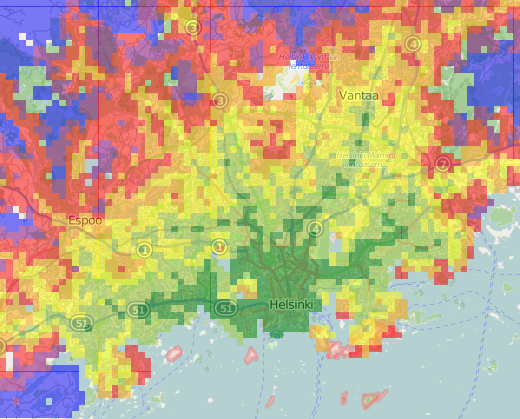
\includegraphics[width=8cm]{images/isarithmic-example.png}
    \caption{An approximated isarithmic map depicting travel times to Helsinki center.}
    \label{fig:isarithmic}
  \end{center}
\end{figure}

\paragraph{Dasymetric Map}

Dasymetric mapping is closely related to choropleth mapping, with the exception that in dasymetric mapping, the enumeration units are not predefined, but rather defined by the data coherency. When creating exact dasymetric maps computationally, the properties can be approximated using a number of techniques, as presented in chapter \ref{subsection:supportedvisualizationmethods}. Dasymetric mapping is most naturally used for data which consists of a set of internally cohesive blocks of area, such as land use (i.e. the distribution of roads, cities, forests etc.) as illustrated in figure \ref{fig:dasymetric}. (Ibid.)

\begin{figure}[htbp]
  \begin{center}
    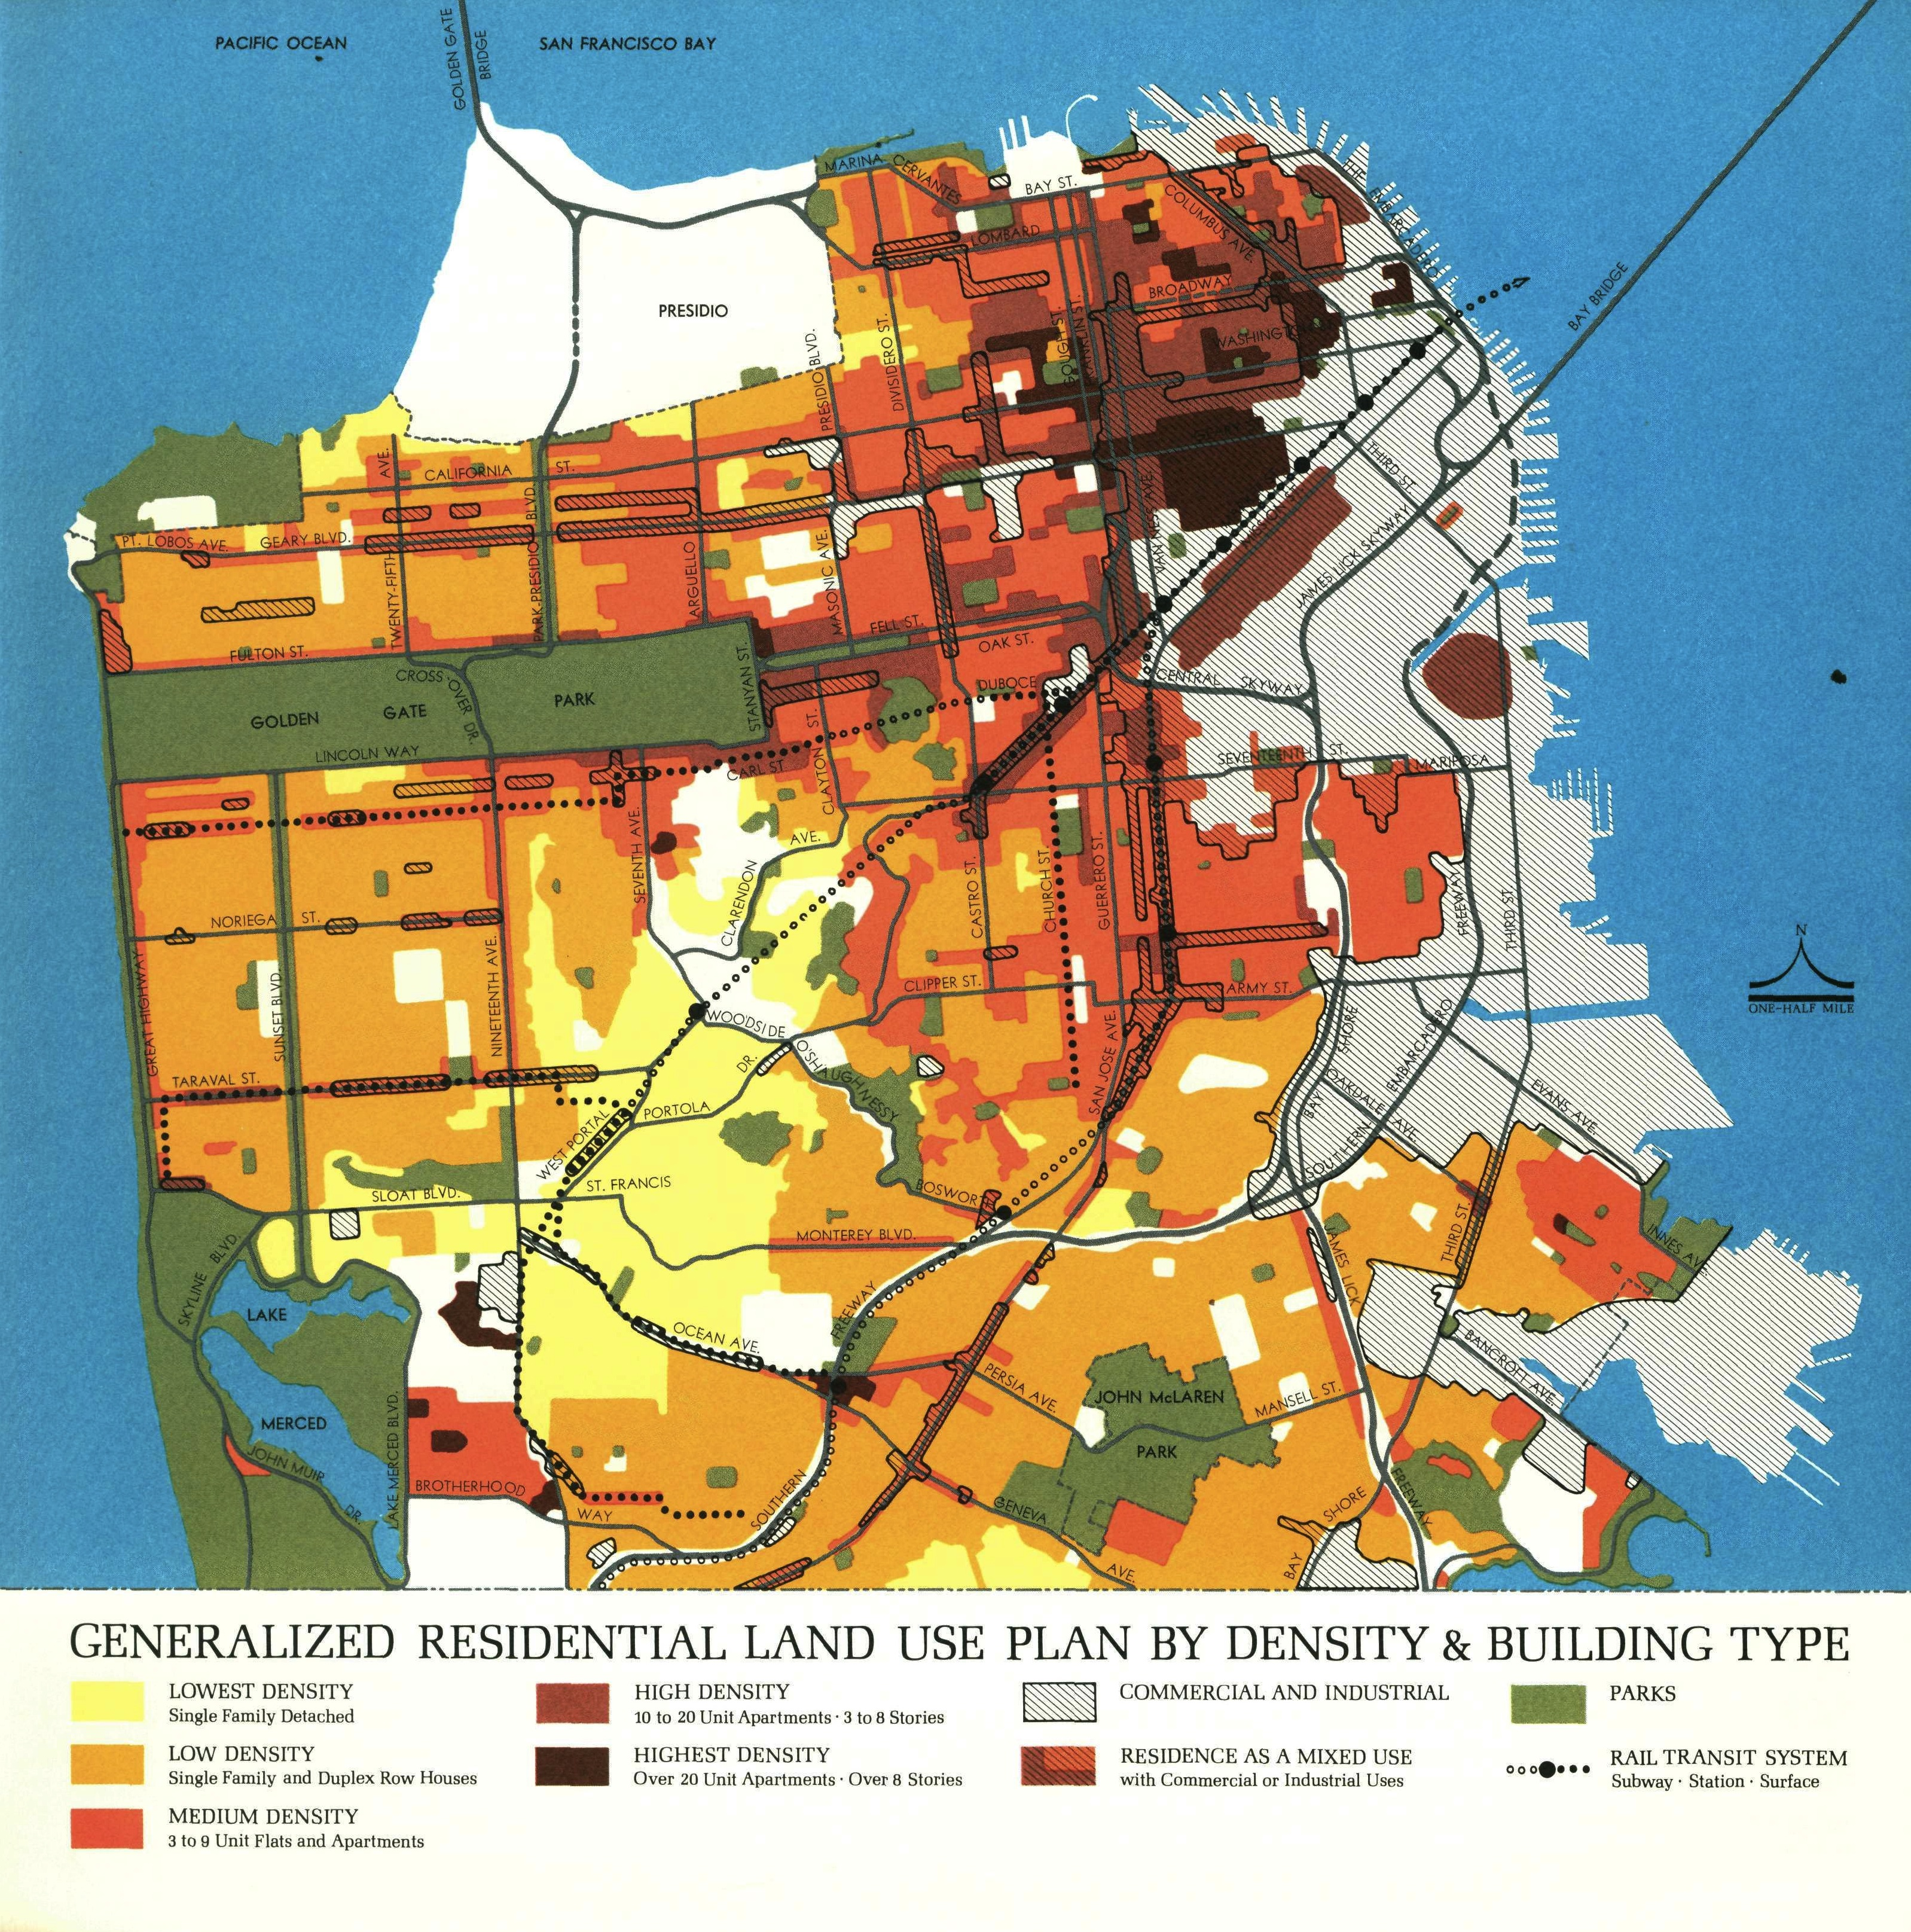
\includegraphics[width=8cm]{images/dasymetric-example.jpg}
    \caption{Dasymetric map depicting land use density in San Francisco \citep{fischer_generalized_2012}.}
    \label{fig:dasymetric}
  \end{center}
\end{figure}

\paragraph{Dot Map}

Dot maps are used to represent data which is associated with locations. With dot maps, the data used can be \emph{true} (truly associated with a single point) or \emph{conceptual} (aggregated to a point). Moreover, dots can be clustered or combined. In practice, dot maps can be used for visualizing, e.g., store locations or the number of homicides in different cities. An example of a dot map is presented in figure \ref{fig:dot}. (Ibid.)

\begin{figure}[htbp]
  \begin{center}
    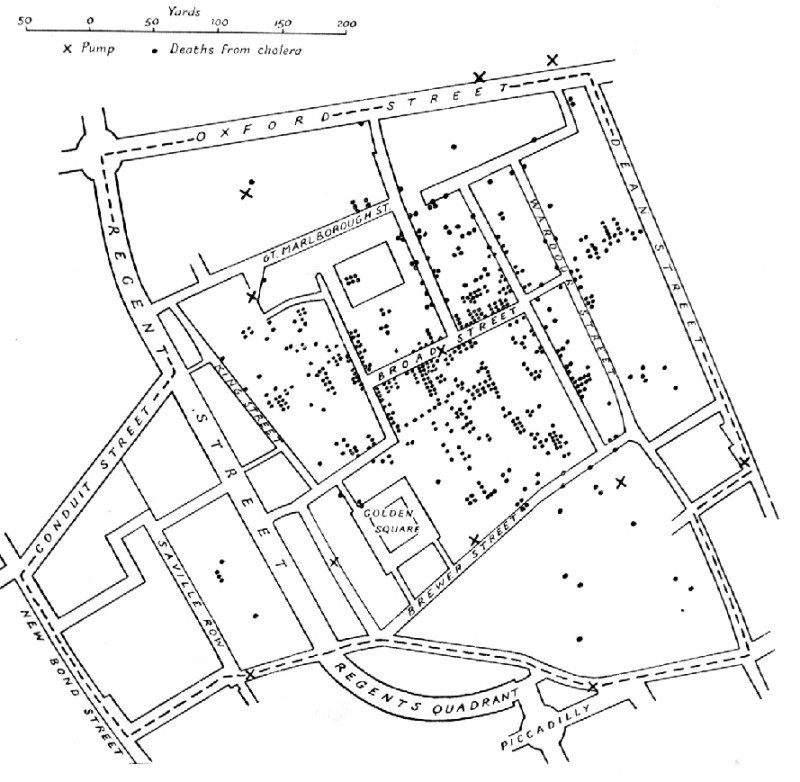
\includegraphics[width=8cm]{images/dot-example.jpg}
    \caption{Dot map depicting cholera cases during the London epidemic of 1854 \citep{snow_cholera_1854}.}
    \label{fig:dot}
  \end{center}
\end{figure}

\paragraph{Proportional Symbol Map}

Proportional symbol maps are closely related to dot maps. They are typically used for visualizing numerical data associated with a location, but unlike with dot maps, the symbols on a map are resized proportionally to the data. Symbols can be geometric or pictorial, and the sizes can be determined using several different methods, e.g., purely mathematical scaling or perceptual scaling which takes human visual inaccuracy into account. An example of a proportional symbol map is presented in figure \ref{fig:proportionalsymbol}. (Ibid.)

\begin{figure}[htbp]
  \begin{center}
    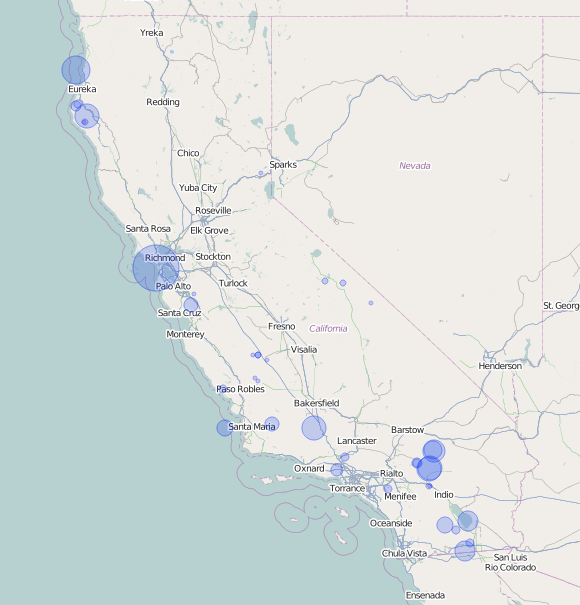
\includegraphics[width=8cm]{images/proportionalsymbol-example.png}
    \caption{Proportional symbol map depicting the magnitude of earthquakes in California.}
    \label{fig:proportionalsymbol}
  \end{center}
\end{figure}

\paragraph{Multivariate Mapping}

Multivariate mapping denotes displaying multiple attributes simultaneously. This can be achieved in several ways. The visualized attributes can be either visualized using a single map or a separate map for each attribute. Additionally, the attributes can be either overlaid (placed on top of each other) or combined (use a single symbol depicting all attributes). (Ibid.) \fixme{add example image}

\paragraph{Cartogram}

Cartograms are used to distort the map based on the data. Thus, cartograms may be used to communicate relative sizes of an attribute in several areas, such as population in each country. This is advantageous when the geographical sizes and attribute values do not correlate, e.g., when some areas with high attribute value are extremely small in size. An example of a cartogram is depicted in figure \ref{fig:cartogram}. (Ibid.)

\begin{figure}[htbp]
  \begin{center}
    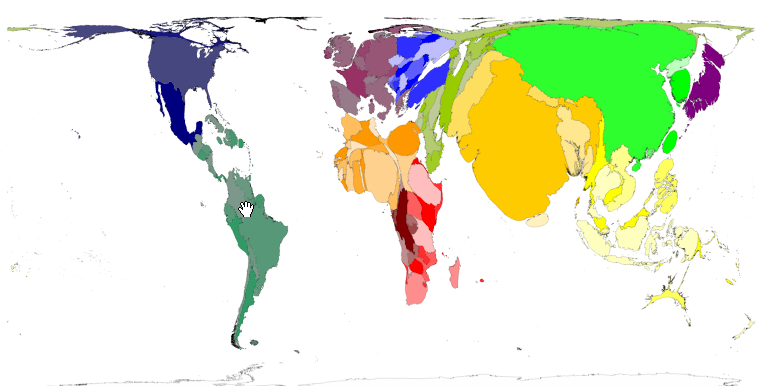
\includegraphics[width=10cm]{images/cartogram-example.png}
    \caption{Cartogram depicting the population of the world \citep{hennig_population_2014}.}
    \label{fig:cartogram}
  \end{center}
\end{figure}

\paragraph{Flow Map}

Flow maps are maps with lines or arrows of varying width from one location to another. Therefore, flow maps excel at displaying movement-related attributes such as immigration from one country to another or wind speed and direction. An example of the flow map is depicted in figure \ref{fig:flow}. (Ibid.)

\begin{figure}[htbp]
  \begin{center}
    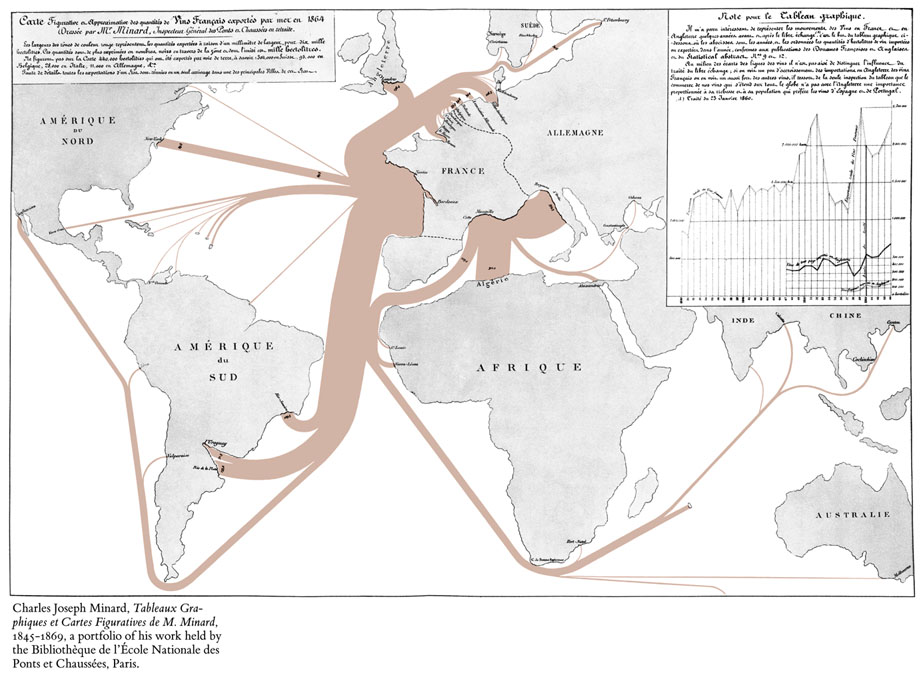
\includegraphics[width=9cm]{images/flow-example.jpg}
    \caption{Flow map displaying the French wine exports in 1864 \citep{minard_carte_1865}.}
    \label{fig:flow}
  \end{center}
\end{figure}

~

Even a single thematic map is often used for multiple different purposes \citep[chap.~2]{schlichtmann_visualization_2002}. For instance, a single map can be read on the \emph{overall level} (``where are the primary schools located in Helsinki metropolitan area?'') and \emph{elementary level} (``is there a primary school in Punavuori?''). Furthermore, some possible uses for a thematic map are ``what is the ratio and distribution of Finnish schools compared to Swedish schools in Helsinki'' or ``what is the spatial distribution of sizes of schools in Helsinki''. Therefore, an efficient map visualization should not lock the user to any single perspective. \fixme{maybe move somewhere? Create a separate (sub)section for interactivity?} \fixme{Interactivity could help here? See \citep{andrienko_interactive_1999}}

\subsection{Effective Thematic Maps}
\label{subsection:effectivemaps}

While the map visualizations adhere to general visualization principles, the principles can be refined by specifying a set of guidelines for maps specifically. \citeauthor{koeman_het_1969} (\citeyear{koeman_het_1969} quoted by \citealt[p.~12]{kraak_cartographic_1998}) defines the guidelines for map visualization process as \emph{``How do I say what to whom''}. \emph{How} refers to the mapping methods and techniques used. \emph{What} refers to the data used and its characteristics. \emph{Whom} refers to the target audience of the visualization. \citet{kraak_cartographic_1998} complements the guidelines with \emph{``and is it effective''}, referring to the self-reflective and iterative nature of visualization.

All the elements above are important to acknowledge when creating a thematic map. While they do not provide an exact formula for determining the effectiveness of a visualization, the elements are incredibly beneficial for creating an effective visualization. Therefore, created visualizations can also be examined with the help of the elements.

~

\fixme{Something about thematic map interactivity \citep[p.~12]{andrienko_interactive_1999,kraak_cartographic_1998} could be relevant in this chapter}

\section{How Thematic Maps Are Made}
\citet{schlichtmann_visualization_2002} describes making thematic maps as a six-step process. The steps are presented below:
\begin{enumerate}
	\item Decide what is the knowledge the viewer should gain from viewing the visualization
	\item Decide on the information to be entered to the visualization
	\item Procure the data needed
	\item Procure a base with the required geometrical characteristics
	\item Select the appropriate graphic means and transcribe the information as necessary
	\item Explain the transcription in a legend
\end{enumerate}

\citet[chap.~1]{slocum_thematic_2014} present an alternative process for thematic visualization. The process consists of five steps and is presented below:

\begin{enumerate}
	\item Consider what the real-world distribution of the phenomenon might look like
	\item Determine the purpose of the map and its intended audience
	\item Collect data appropriate for the map's purpose
	\item Design and construct the map
	\item Determine whether users find the map useful and informative
\end{enumerate}

In practice, the processes described by \citeauthor{schlichtmann_visualization_2002} and \citeauthor{slocum_thematic_2014} concentrate on different perspectives of thematic mapping. \citeauthor{schlichtmann_visualization_2002} begins the process by defining the goal of the visualization while \citeauthor{slocum_thematic_2014} provides a more data-centric approach starting with phenomenon definition. Unlike \citeauthor{schlichtmann_visualization_2002}, \citeauthor{slocum_thematic_2014} emphasizes an iterative approach of the visualization. In both processes, defining and designing the visualization is emphasized, the actual visualization (turning the data into visual representation) being addressed in only one of the steps.

\citet[chap.~1]{slocum_thematic_2014} express their concern on the utilization of the processes defined above. According to them, it is likely that naive visualizers do not follow the steps, but take shortcuts when designing the visualizations, resulting in subpar visualizations. Therefore, it is often needed to nudge the visualizers towards using (one of) the processes when building a visualization.

The steps are used to produce a visual representation (graphic) of the data. Additionally, \citet{schlichtmann_visualization_2002} identifies several objectives for the resulting graphic, presented in table \ref{table:geovisualizationobjectives}.

\LTcapwidth=\textwidth
\begin{longtable}{|p{3cm}|p{10cm}|}
\hline
\textbf{Name} & \textbf{Description} \\ 
\hline
Clarification & Making the map clear and readable. In practice, this means that the topemes (symbols) in a map should be easily detectable and distinguishable from each other \\
\hline
Emphasis & Making topemes and other important characteristics of the visualization to stand out visually \\
\hline
Types of Entries & Having a clearly distinguishable type for each topeme. \\
\hline
Sets of Types & Grouping data points and symbols with similar traits in order to make them belong together visually. Ideally, the visual similarity should be related to the conceptual similarity. \\
\hline
Cross-Relations & Visually indicating the potential relations and similarities between different types or between entries of different types. \\
\hline
Local Syntax & Aligning visual properties of the topemes to prevent unintentional emphasis of single topemes. \\
\hline
Local Ensembles & Supporting topemes with multiple properties (such as the numbers of children and adults in an area) so that the topeme visually reflect both the individual properties and the combination of all properties. \\
\hline
Multilocal Ensembles & Supporting topemes with multiple geographical properties (such as spatial distribution of people)  \\
\hline
Addable and Non-Addable Quantities & Differentiating addable and non-addable properties. Typically absolute quantitative properties are addable while relative and qualitative properties are non-addable. Addable properties should be visualized in a way that cognitively supports addition (e.g., with sizes of elements) while non-addable quantities should be visualized without said feature (e.g., with colors.) \\
\hline
The Surface Illusion & Creating an illusion of surface on the map. This can be achieved for example by using illumination and shadowing. These visual traits can convey a meaning themselves and often naturally do so. \\
\hline
\caption{Map visualization objectives as per \citet{schlichtmann_visualization_2002}}
\label{table:geovisualizationobjectives}
\end{longtable}


The objectives above are important when visualizing geographical data on a map. Therefore, it is needed to take those into account when creating a visualization tool in order to enable or even encourage the visualizers to reach as many of the objectives as possible.

\chapter{Software Reuse}
\label{chapter:reuse}

In order to create a reusable software framework for visualization, it is necessary to study software reuse along with different reuse techniques and their characteristics, advantages and disadvantages.

\citet{krueger_software_1992} presents software reuse as a process of reusing existing software code (applications, libraries, functions or single lines) when building new software, while according to \citet{mohagheghi_empirical_2008}, reuse is not restricted to code, but can also refer to other software assets such as design. However, both agree that software reuse combines several different existing pieces of code (and possibly other assets) along with new assets which are specific for the application in question. According to \citet{mcilroy_mass-produced_1969} and \citet{boehm_managing_1999}, it is one of the most effective techniques of reducing the development time and cost of complex software products.

\section{Software Reuse Advantages \& Disadvantages}

When used appropriately, software reuse has several benefits. In their overview of multiple case studies, \citet{mohagheghi_empirical_2008} discovered that in most cases, using reused software components resulted in a considerably lower number of software defects and better productivity. Several of the studies implied that reusing software is also beneficial for software complexity and product time-to-market. However, it should be noted that since the overview only addresses case studies, its results should not be considered universally applicable.

Although reusing software is often said to decrease the effort needed \citep{mcilroy_mass-produced_1969, boehm_managing_1999, mohagheghi_empirical_2008} \fixme{there must be many more sources for this available}, concrete evidence for this is difficult to find \citep{mohagheghi_empirical_2008}.

Given its lucrative advantages, software reuse is definitely beneficial for many software systems. However, according to \citet{krueger_software_1992}, software reuse can be problematic and even disadvantageous. Learning to use a specific piece of reusable software often takes considerable effort. Moreover, finding suitable code fragments may also prove to be a challenge. For uncomplicated software systems and especially reusable components, it may not be worth the effort. Therefore, developer needs to carefully consider all sides of reusing when building a software system; according to \citet[chap.~1.3]{krueger_software_1992}, for successful software reuse scenario, the amount of intellectual effort between the concept and implementation of the system must be as low as possible. In practice, this means that the value of the reused component must be as high as possible for the developed system, while the implementation cost (resources needed to take the reusable component into use) should be relatively low. 

\section{Factors for Successful Software Reuse}
\label{section:successfullreusefactors}
\citet{frakes_success_1994} present six critical factors for successful software reuse: management, measurement, legal, economics, design for reuse, and libraries. Some of the factors are relevant only for a corporate-level reuse program, but many are critical for smaller scale reuse as well.

Successful reuse requires the \textbf{management} to commit to a long-term, top-down support, because reusing software may require years to pay off the costs. Also, \textbf{measurement} of reuse is vital to reuse software successfully. Both \emph{reuse level} (the ratio of reused software to total software) and \emph{reuse factors} (things affecting the increase of reuse) should be measured.

\textbf{Legal} issues are also important to consider when reusing software. Specifically, the rights and responsibilities of providers and consumers of reusable software should be agreed on. Moreover, using software with conflicting licenses may cause problems.

\textbf{Economics} present a challenge in systematic reuse scenarios. Measuring reuse costs is not straightforward as often costs of creating a reusable component are compensated by benefits in some other project using the component.

In order to \textbf{design for reuse}, a degree of domain knowledge is required. This necessitates the study of the domain when creating a \emph{domain-specific} reusable software. In addition to that, reusable software design requires effort on encapsulation, abstraction and interfaces.

Lastly, reusable software \textbf{libraries} are required to fully benefit from the reusability effort. Libraries enable storing, retrieving and finding the reusable software.

\section{Analyzing Software Reuse}
According to \citet{krueger_software_1992}, in order to analyze reusing software, the reuse process to be studied should be separated into four \emph{dimensions}. The dimensions are presented below.

~

\paragraph{Abstraction} is the process of making a piece of software more generic, thus making it applicable to a wider range of software projects. Software reuse is almost always based on abstraction, but according to \citet{krueger_software_1992}, raising the abstraction level has proven to be difficult, thus making building reusable software a nontrivial process.

\paragraph{Selection} facilitates finding, comparing and choosing suitable pieces of software. For example, libraries or frameworks aid selection by bundling and structuring the software components.

\paragraph{Specialization} is the process of making the abstracted component more specific, usually by parameterizing the software or making it transformable.

\paragraph{Integration} facilitates providing the software with reusable components, for example with a mechanism to import relevant modules or functions to the software.

\section{Software Reuse Methods}

Software reuse is not a single, uniform procedure or technique. Several different reuse techniques exist to cater different needs. Consequently, different reuse methods excel at different areas. In order to describe the advantages and disadvantages of the methods, we describe the using the reuse dimensions presented in the previous section.

\citet{krueger_software_1992} and \citet{johnson_frameworkscomponents+_1997}, among others, present and analyze software reuse methods. From these, we have selected the most relevant for web environment, presenting those below.

\subsection{High-Level Languages}
High-level languages denote programming languages which are designed to be on a high abstraction level and thus contain features which are not necessary for a programming language but benefit or speed up the development. Traditional examples of these kind of features are automatic memory allocation \citep{krueger_software_1992} and language constructs such as exceptions \citep{mitchell_concepts_2003}. More modern high-level language features are value type checking systems and abstracted support for parallel operations using futures \citep{totoo_haskell_2012}. It should be noted that the high-levelness of a language is a \emph{relative} property, i.e., it is not possible to determine the requirements for a high-level language per se, only high-levelness of languages compared to other languages. For example, \citet{krueger_software_1992} considers all programming languages above the abstraction level of the assembly language high-level languages, while \citet{carro_high-level_2006} consider e.g., lack of automatic memory management or type system a sign of lower-level language.

High-level languages \emph{abstract} frequently used procedures into seemingly uncomplicated operations, thus reducing the work and cognitive capacity needed for developing the application. \citep[chap.~3]{krueger_software_1992}

As the number of elementary high-level language constructs is usually relatively low it is possible for programmers to master the use of those constructs with sufficiently little effort, rendering \emph{selection} unproblematic. \citep[chap.~3]{krueger_software_1992}

\emph{Specialization} of high-level language features is usually achieved by parameterizing the constructs, either implicitly or explicitly. For example, when instantiating a class in Java, the only parameterization needed for memory management is the actual object instance. However, e.g., exception handling always requires at least the logic needed for handling the exception. \citep[chap.~3]{krueger_software_1992}

\emph{Integration} of high-level language features is automatically done when compiling the software code. However, due to the nature of high-level languages, it is usually not possible to mix-and-match different programming languages easily in the same program. \citep[chap.~3]{krueger_software_1992}

The advantages of high-level languages are mainly related to the decreased need for developing frequently needed procedures manually, such as allocating or deallocating memory, case-by-case. These operations in high-level languages can be mapped into more complex procedures in some lower-level languages, effectively making them reusable software components. In practice, using high-level languages can yield a productivity gain up to 500 \%. \citep[chap.~3]{krueger_software_1992}

The main disadvantage of using high-level languages is the potential decrease in performance. As with any software reuse, high-level programming languages abstract the supported procedures by making them more generic. This often leads to additional complexity and unnecessary operations on the compiled program. However, the decrease can often be minimized by using additional compile-time optimizations. \citep{carro_high-level_2006}

On the web, the technologies used on the client-side are inherently fixed to descendants of HyperText Markup Language (HTML), Cascading Style Sheets (CSS) and JavaScript \citep{world_wide_web_consortium_html5_2014,world_wide_web_consortium_cascading_2011,ecma_ecmascript_2011}. Therefore, web application languages are relatively high-level by definition. However, it is still possible to raise the abstraction level by using e.g., CoffeeScript \citep{ashkenas_coffeescript_2009} instead of JavaScript or LESS \citep{sellier_less_2009} instead of CSS.

\subsection{Design and Code Scavenging}

Design and Code scavenging refers to the technique of scavenging pieces of software \emph{ad hoc} from existing software systems and using the pieces as parts for a new software system  \citep[chap.~4]{krueger_software_1992}. The aim of this technique is to reduce the amount of work needed to build the system. For example, when building an user interface (UI) component for choosing a date, the developer may scavenge the code for a calendar from an older software system.

Scavenging can be done without modifications to the code in the target code base (code scavenging) or by modifying the details of the scavenged code (design scavenging) \citep[chap.~4]{krueger_software_1992}. The \emph{abstraction} gained by scavenging is therefore mostly informal and in some cases even its existence is questionable \citep[chap.~3]{sametinger_software_1997}. Usually, there is no ``hidden part'' of the abstraction but the developer must maintain the functionality of all the code himself \citep[chap.~3]{sametinger_software_1997}.

Usually there is no formal mechanism or support for \emph{selecting} pieces of software to be scavenged. Therefore, the developer must rely on his memory, experience and word-of-mouth in order to find suitable pieces of software. \citep[chap.~3]{sametinger_software_1997}

\emph{Specialization} is done by manually editing the scavenged source code. While it is often the fastest method of acquiring results, this requires the developer to deeply understand the scavenged implementation. It can also lead to fragmentation and maintainability issues in the future. \citep[chap.~4]{krueger_software_1992}

\emph{Integration} of the scavenged code is done by copying and pasting the code to the target source code file. This may lead to namespace collisions between original and scavenged code which may result in the need for refactoring the code. \citep[chap.~4]{krueger_software_1992}

The main advantages of design and code scavenging are the ability to quickly include existing functionality to new software systems \citep[chap.~4]{krueger_software_1992}. As it is usually not needed to prepare the code to be scavenged before scavenging it, the extent of possible pieces of software is often significantly larger than when using any other reuse method. 

However, finding suitable pieces of software for scavenging is hard. Moreover, scavenging pieces of software often does not decrease the \emph{cognitive distance} between the target and implementation of the system. It may also create issues with maintainability of the software. \citep[chap.~4]{krueger_software_1992}

\subsection{Source Code Components}

Using source code components is a type of reuse that chooses and uses software components from a component repository \citep[chap.~3]{sametinger_software_1997}. Software component can be any piece of code, but in practice, components usually consist of one or more functions, modules or classes \citep[chap.~3]{sametinger_software_1997}. An example of a source code component is a trigonometry module which contains functions for sine, cosine and tangent calculations. When a developer needs to calculate sines in her program, she searches a component repository for trigonometry components and utilizes the component found in her own program \citep[chap.~5]{krueger_software_1992}.

Ideally, source code components \emph{abstract} the implementation details of the component inside. This means that the required cognitive distance between the concept and the implementation of the software system is lower when using source code components instead of e.g., code scavenging. 

In order to be \emph{selectable}, source code components should be accompanied by abstract names (function names) and descriptions of the functionality provided \citep[chap.~5]{krueger_software_1992}. The names should describe \emph{what} the components does instead of \emph{how} it does it \citep[chap.~5]{krueger_software_1992}. These names can then be used for reasoning about the purpose of the component and finding the component in source code component repositories -- in order to use the component, the developer must be able to find it and to know what it does \citep[chap.~5]{krueger_software_1992}.

Source code components can be \emph{specialized} by modifying the source code \citet[chap.~5]{krueger_software_1992}. However, as this technique yields unwanted consequences explained in the previous section, many components support specialization by parameterization. For example, the programmer could provide the sine function the angle in question. Additionally, when integrating the trigonometry module to her software system, the programmer could specify if the functions should use degrees or radians. In some components, specialization can also be achieved via subclassing \citep[chap.~5]{krueger_software_1992}.

All modern programming languages support \emph{integration} of reusable source code components written in the same language. Usually, the procedure is a very simple addition of source code files, which requires little to no effort on the programmer side. However, all source code components can't be used in the same program due to conflicts e.g., in naming and value types \citep[chap.~5]{krueger_software_1992}.

The main advantages of using source code components are the abstraction provided and organized nature of the component repositories. Ideally, the repositories provide a search functionality so that even developers with no previous experience on the component domain can find the components needed. Moreover, the abstraction level and the hiding of implementation details decreases the cognitive distance between the concept and the implementation of the system and reduce the source code needed to be written.

The main disadvantages of the source code components lie in the fact that the functionality must be deliberately designed to support reuse. The abstraction of the components is a major challenge \citep[chap.~5]{krueger_software_1992} in designing source code components. Additionally, the component repositories need administration and maintenance.

\subsection{Software Schemas}

\fixme{Add similarly structured content as in the previous subsubsection. Or maybe drop?}

\subsection{Application Generators}

Application generators are usually domain-specific generators which take very high level instructions (specifications) as input and then output significantly lower level software code (implementation) \citep[chap.~7]{cleaveland_building_1988,krueger_software_1992}. On fundamental level, application generators differ from high-level language compilers mainly by being designed to work on a narrow domain and thus being able to support considerably higher-level instructions \citep[chap.~7]{krueger_software_1992}. Unlike source code components, the reused components generated by application generators are usually not encapsulated or separated \citep[chap.~3]{sametinger_software_1997}.

Application generators \emph{abstract} the concept or specification of the software system, hiding the actual implementation completely from the user of the generator \citep{cleaveland_building_1988}. However, in some cases it may be necessary to modify the output of the generator which essentially removes the abstraction.

In principle, \emph{selecting} application generations is moderately easy since the abstraction level of application generators is usually very high, rendering reasoning about the purpose of the generator fairly easy \citep[chap.~7]{krueger_software_1992}. However, since application generators are usually suited for a very narrow domain, it is usually difficult to find a suitable generator \citep[chap.~7]{krueger_software_1992}.

Typically, software systems generated with application generators consist of variant and invariant parts \citep[chap.~7]{krueger_software_1992}. Invariant part is the part of the program which the developer using the generator can't modify. The developer \emph{specializes} the program by modifying the variant part. There are several methods of modifying the variant part. One of the simplest may be straightforward parameterization: the developer chooses the parameters of the system from a predefined set of alternatives. This method makes using the generation extraordinarily easy. However, it also limits the resulting application considerably.

On the other end of the spectrum, the application generator may require the variant parts to be inputted using a domain-specific or generic-purpose programming language. This makes the application generator incredibly versatile, but requires both more domain-specific and programming knowledge.

Typically, application generators generate complete applications which do not require further \emph{integration} \citep[chap.~7]{krueger_software_1992}. However, occasionally, the resulting applications are not independent per se, but require integration to other systems. This may be an issue since often it is not possible to select the integration interfaces freely, but to use the ones provided by the generator.

One of the main advantages of the application generators is the abstraction they provide. In some cases, the application generators may even require no programming language knowledge as long as the user has relevant domain-specific knowledge \citep{horowitz_survey_1985}. Moreover, application generators excel when there is a need for building multiple similar applications \citep[chap.~7]{krueger_software_1992}. 

However, application generators require an unambiguous mapping between the specifications and implementation details \citep[chap.~7]{krueger_software_1992}. Moreover, building application generators requires a reliable, generic implementation and user interfaces for developers \citep{cleaveland_building_1988}. Therefore, building application generators requires comprehensive domain-specific knowledge in addition to extensive software development expertise.

\subsection{Design Patterns}

\fixme{Add similarly structured content as in the previous subsubsection}

\subsection{Software Frameworks}

Software frameworks are a reuse technique which combines the use of software components and programming patterns \citep{johnson_frameworkscomponents+_1997}. Therefore, it can be argued that software frameworks enable creating reusable software design. Another definition of software frameworks is a collection of consolidated components, i.e., components which share the design, interfaces, and, to some degree, implementations \citep{johnson_frameworkscomponents+_1997}. It should also be noted that software frameworks are typically strictly object-oriented reuse technique \citep{johnson_frameworkscomponents+_1997}.

Largely, software frameworks \emph{abstract} the implementation details the same way that components do, i.e., providing a higher-level interface for the low-level operations. In addition to that, frameworks abstract software \emph{design patterns} used to provide a more complete architecture and functionality.

\emph{Selection} of frameworks can be regarded as straightforward, since typically, the number of applicable frameworks is considerably smaller than, e.g., the number of applicable source code components. However, as frameworks are by definition more complex than single software components \citep{johnson_frameworkscomponents+_1997}, selecting the right framework of a purpose may be considerably more difficult \citep{fayad_enterprise_2000}.

\emph{Specializing} frameworks is greatly dependent on the purpose and design of the framework. As some frameworks are designed as domain-specific \citep{johnson_frameworkscomponents+_1997}, it is typically not needed to specialize the system extensively. According to \citet{brugali_framework_1997}, frameworks are usually specialized in an object-oriented fashion: using parameters and subclasses to fine-tune functionality \citep{brugali_framework_1997}.

Typically, software frameworks are \emph{integrated} to other frameworks and to larger software systems. However, as frameworks are generally designed for adaptation instead of integration \citep{mattsson_framework_1999}, this leads to integration problems. \citet{mattsson_framework_1999} describe several framework integration problems, e.g., architecture, design and pattern mismatches. Nonetheless, most of the problems can be overcome by using a number of solutions, such as separating the concerns cleanly and wrapping the functionality to compliant components \citep{mattsson_framework_1999}.

One of the main advantages of frameworks is that they enable a complete, potentially opinionated approach for reusing software while preserving the possibility for customization \citep{johnson_frameworkscomponents+_1997}. The main disadvantages of using software frameworks consist of occasional steep learning curve and challenges in integration \citep{fayad_object-oriented_1997}.

\chapter{Research Gap}
\label{chapter:researchgap}

Currently, research on geographic or map visualization is abundant \fixme{Use a bunch of geoviz references to prove this? Or some other way?}. Moreover, according to the visualization definition by \citet{kosara_visualization_2007}, it may be possible to abstract parts of the visualization implementation in order to achieve visualization process which requires less effort and technical knowledge. However, both research about geovisualization-related software reuse and actual reusable geovisualization components are scant. This implies that there is room for improvement in both research and implementation related to geovisualization software.

To address this shortcoming, we decided to attempt creating a reusable geovisualization tool for the web. We also evaluated the tool in order to obtain knowledge about its benefits when compared to building geographic visualizations from the beginning.

\fixme{IMHO this is a bit too short for a chapter. How to fix?}
